\documentclass{article}
\usepackage{blindtext}
\usepackage[a0paper, landscape, margin=1in]{geometry}

%usepackage[utf8]{inputenc}
%usepackage[english]{babel}
\usepackage[english,spanish]{babel}
\usepackage[latin1]{inputenc}

\usepackage{multicol}
%usepackage{tasks}

\usepackage{wrapfig}
\usepackage[table,xcdraw]{xcolor}
\usepackage{caption}

\usepackage[pdftex]{graphicx}

\usepackage{hyperref}

%usepackage{amssymb}
\usepackage{amsmath}
%usepackage{mathtools}
%usepackage{zed-csp}
%usepackage{amsthm}
\usepackage{numprint}
\usepackage{nicefrac}
%usepackage{relsize}
\usepackage{listings}
%usepackage{chngcntr}

\newtheorem{theorem}{Teorema}[section]
\newtheorem{heuristic}[theorem]{Heur\'istica}

\lstdefinelanguage{sql}{
 alsodigit = {-},
 morecomment=[l]{--}, % l is for line comment
 morecomment=[s]{/*}{*/}, % s is for start and end delimiter
}

\lstset{
	language={sql},
	%numbers=left,
	%breaklines=true,
	backgroundcolor=\color{black!10},
	tabsize=2,
	%\basicstyle=\tiny,%\ttfamily,
	%literate={\ \ }{{\ }}1
	commentstyle=\color{gray}
}

\hypersetup{
	%frenchlinks=true,
	linktocpage=true,
	colorlinks=false,
	%linkcolor=tec,%=red,%black!40,
	%citecolor=tec,%=red,
	%filecolor=tec,%black,
	%urlcolor=tec,%black,
	%linkbordercolor={.89 .13 .21},
	%citebordercolor={.41 .85 .15},
	%urlbordercolor={0 0 1},
	pdftitle={Propuesta de dise\~no de un sistema de informaci\'on para la producci\'on y an\'alisis de datos referentes al presupuesto del MEP por nivel educativo} %,
	%pdfpagemode=FullScreen
}

\graphicspath{{img/}}

\begin{document}
\begin{multicols}{6}[]

\title{Propuesta de dise\~no de un sistema de informaci\'on para la producci\'on y an\'alisis de datos referentes al presupuesto del MEP por nivel educativo}

\author{
	Wilberth Castro \\
	\small{\texttt{wilz04@gmail.com}}
}

\date{\small{22 de mayo 2023}}

\maketitle


\begin{abstract}
	En este documento se describe el dise\~no de un sistema de informaci\'on mediante el que ser\'a posible implementar un proceso de planificaci\'on de presupuesto por resultados para el Ministerio de Educaci\'on P\'ublica de Costa Rica. En este documento (1) se describe la naturaleza de los datos que procesar\'a el sistema de informaci\'on y el prop\'osito en la toma de decisiones que tendr\'a su procesamiento (2) se discute a cerca del proceso de carga de datos en el sistema de informaci\'on, de los encargados del procesamiento y reporte de los datos, y de la frecuencia de cada proceso, (3) se definen las herramientas mediante las que se realizar\'a el procesamiento y an\'alisis de datos, y el despliegue de los reportes, (4) se propone una serie de indicadores que podr\'an ser calculados a partir de los datos procesados por el sistema de informaci\'on. Los insumos necesarios para la producci\'on de este documento han sido recopilados mediante una serie de actividades organizadas en conjunto con las direcciones y dependencias del Ministerio de Educaci\'on P\'ublica de Costa Rica.
\end{abstract}

% --------------------------------------------------------------------------------------------------------------------------------
\section{Introducci\'on} \label{sec:intro}

En este documento se describe el dise\~no de un sistema de informaci\'on mediante el que ser\'a posible implementar un proceso de planificaci\'on de presupuesto por resultados para el Ministerio de Educaci\'on P\'ublica de Costa Rica. En general, la planificaci\'on de un presupuesto por resultados requiere de una serie de actividades similar a la siguiente. El sistema de informaci\'on descrito aqu\'i deber\'a permitir la automatizaci\'on, hasta donde sea posible, de cada actividad en la serie.

\begin{enumerate}
	\item Identificaci\'on de los objetivos estrat\'egicos: Lo primero que se debe hacer es identificar los objetivos estrat\'egicos que se quiere alcanzar. Los objetivos estrat\'egicos deben ser espec\'ificos, medibles, alcanzables, todo esto en un plazo determinado. Por ejemplo, algunos objetivos estrat\'egicos podr\'ian ser \emph{mejorar la calidad educativa}, \emph{aumentar la cobertura educativa} o \emph{reducir la brecha educativa entre distintos grupos de la poblaci\'on}.

	\item Identificaci\'on de las metas: Una vez que se han establecido los objetivos estrat\'egicos, es necesario definir las metas que permitir\'an medir el progreso hacia tales objetivos. Las metas deben ser espec\'ificas y cuantificables. Por ejemplo, si el objetivo estrat\'egico es \emph{mejorar la calidad educativa}, una meta podr\'ia ser \emph{aumentar en un 10\% el porcentaje de estudiantes que obtienen calificaciones de excelencia en las pruebas estandarizadas}.

	\item Asignaci\'on de recursos a las metas: Una vez que se han identificado las metas, es necesario determinar una asignaci\'on de recursos que permita alcanzarlas. Los recursos deben ser asignados de manera proporcional a la importancia de cada meta y a su impacto en la consecuci\'on de los objetivos estrat\'egicos. Para ello, se pueden utilizar diferentes criterios de asignaci\'on, como el costo de implementaci\'on, la prioridad, el impacto esperado o la urgencia de la meta.

	\item Establecimiento de indicadores de resultados: Finalmente, es necesario establecer indicadores que permitan medir el progreso y los resultados obtenidos en relaci\'on a las metas y los objetivos estrat\'egicos. Estos indicadores deben ser claros, precisos y estar alineados con los objetivos estrat\'egicos y las metas definidas previamente.
\end{enumerate}

Es importante tener en cuenta que el proceso de asignaci\'on de recursos basado en resultados es un proceso iterativo que requiere revisi\'on y ajuste continuo a lo largo del tiempo. Adem\'as, es fundamental contar con informaci\'on y datos precisos y actualizados para tomar decisiones informadas y garantizar una asignaci\'on de recursos efectiva.

% --------------------------------------------------------------------------------------------------------------------------------
\section{Lista preliminar de indicadores}

El cuadro \ref{tab:matrix} contiene la lista preliminar de indicadores. La lista fue proveida por el Viceministro de Planificaci\'on Institucional y Coordinaci\'on Regional del MEP.

\begin{center}
	\captionof{table}{Lista preliminar de indicadores.}
	\label{tab:matrix}
	\rowcolors{2}{gray!20}{gray!10}
	\begin{tabular}{p{0.1\linewidth}p{0.8\linewidth}}
		\rowcolor{gray!40}
		N & Indicador \\
		%hline
		1 & Centros educativos por modalidad 2023 \\
		2 & Estudiantes por centro educativo 2023 \\
		3 & Docentes por centro educativo 2023 \\
		4 & Personal administrativo por centro educativo 2023 \\
		5 & Centros educativos con comedores estudiantiles 2023 \\
		6 & Beneficiarios de comedores estudiantiles por centro educativo 2023 \\
		7 & Centros educativos que reciben dos o m\'as tiempos de alimentaci\'on 2023 \\
		8 & Centros educativos con transporte estudiantil 2023 \\
		9 & Beneficiarios de transporte estudiantil por centro educativo 2023 \\
		10 & Centros educativos con huertas escolares 2023 \\
		11 & Monto anual 2023 asignado de la ley 6746 por centro educativo \\
		12 & Centros educativos urbanos 2023 \\
		13 & Centros educativos rurales 2023 \\
		14 & Centros ind\'igenas 2023 \\
		15 & Centros educativos unidocentes \\
		16 & Centros educativos cient\'ificos \\
		17 & Centros educativos human\'isticos \\
		18 & Centros educativos privados 2023 \\
		19 & Centros educativos con conectividad \\
		20 & Matr\'icula por Direcci\'on Regional \\
		21 & Centros educativos por direcci\'on regional \\
		22 & Supervisores por direcci\'on regional \\
		23 & Centros educativos con orden sanitaria \\
		24 & Presupuesto MEP 2010-2023 \\
		25 & Presupuesto FEES 2010-2023 \\
		26 & Presupuesto de otras instituciones 2010-2023 \\
		27 & Presupuesto MEP por partida 2010-2023 \\
		27.1 & Remuneraciones Y Conexos \\
		27.2 & Servicios \\
		27.3 & Materiales Y Suministros \\
		27.4 & Bienes Duraderos \\
		27.5 & Transferencias Corrientes \\
		27.6 & Transferencias De Capital \\
		28 & Presupuesto por programa presupuestario \\
		29 & Ejecuci\'on presupuestaria total por a\~no 2010-2022 \\
		30 & Inversi\'on en comedores total 2010-2023 el dato por a\~no \\
		31 & Inversi\'on en transporte estudiantil total 2010-2023 el dato por a\~no \\
		32 & Estudiantes excluidos por centro educativo 2021-2022-2023 \\
		33 & Total de Estudiantes graduados de secundaria por centro educativo 2010-2022 \\
		34 & Estudiantes graduados de secundaria Acad\'emica por centro educativo 2010-2022 \\
		35 & Estudiantes graduados de secundaria t\'ecnica por centro educativo 2010-2022 \\
		36 & Estudiantes graduados de secundaria biling\"ue por centro educativo 2010-2022 \\
		37 & Estudiantes graduados de secundaria nocturna por centro educativo 2010-2022 \\
		38 & Estudiantes graduados de secundaria abierta para adultos por centro educativo 2010-2022 \\
		39 & Cantidad de docentes por edad simple 2023 \\
		40 & Cantidad de docentes interinos 2023 \\
		41 & Cantidad de cocineras nombradas por el MEP 2023 \\
		42 & Cantidad de cocineras nombradas por las juntas 2023 \\
		43 & Investigaciones del Departamento de Estudios e Investigaci\'on Educativa (DEIE) de la Direcci\'on de Planificaci\'on Institucional \\
		44 & Centros educativos con laboratorio de inform\'atica \\
		45 & Centros educativos ubicados en los distritos de mayor incautaci\'on de tr\'afico de drogas \\
		46 & Centros educativos ubicados en los distritos de mayor incidencia de homicidios \\
		47 & Centros educativos ubicados en distritos de IDS MUY BAJO \\
		48 & Centros educativos ubicados en distritos de IDS BAJO \\
		49 & Centros educativos ubicados en distritos de IDS MEDIO \\
		50 & Centros educativos ubicados en distritos de IDS ALTO \\
		51 & Centros educativos ubicados en distritos de IDS MUY ALTO
	\end{tabular}
\end{center}

% --------------------------------------------------------------------------------------------------------------------------------
\section{Naturaleza de los datos que procesar\'a el sistema de informaci\'on} \label{sec:data}

% Descripci\'on de los datos que permitir\'a procesar la herramienta y qu\'e prop\'osito tendr\'an en la toma de decisiones.

En la planificaci\'on de un presupuesto por resultados, para cada objetivo estrat\'egico es necesario dise\~nar uno o varios programas que permitan satisfacer el objetivo estrat\'egico, mediante los que las actividades puedan ser realizadas y a los cuales sea posible asignar presupuesto. Sin embargo, en Costa Rica, los centros educativos reciben fondos no solo por parte del ministerio, los fondos de cada centro provienen tambi\'en de otras fuentes de ingreso, algunas establecidas por ley. El consumo de los fondos de cada centro est\'a a cargo de una junta semiaut\'onoma, y existen leyes que dificultan la reducci\'on del presupuesto, de los fondos que se transfiere cada a\~no a los centros, por lo que la implementaci\'on de un juego de programas diferente del actual mediante el que sea posible mejorar significativamente la situaci\'on actual es m\'inimamente plausible.

Una estrategia de planificaci\'on adecuada para el ministerio podr\'ia consistir en una variante de la descrita anteriormente, podr\'ia consistir en la implementaci\'on de una herramienta que permita la transmisi\'on de los objetivos estrat\'egicos a lo largo de todo el organigrama del ministerio\footnote{Actualmente hay una interrupci\'on del flujo, las juntas no tienen acceso al sistema en el que se registran los objetivos del ministerio.}, que disponga de los datos necesarios para el c\'alculo de los indicadores, que facilite el monitoreo del consumo de los fondos en tiempo real, incluyendo el consumo de los fondos de los centros educativos, y que permita registrar nuevas actividades en los programas existentes.

Cada centro educativo es administrado por una ``junta'' semiaut\'onoma. Cada junta se encarga de consumir los fondos como corresponda para el centro educativo que administra, y de reportar mensualmente al ministerio el consumo de los fondos. Actualmente, para esto se utiliza una hoja de c\'alculo, sin embargo, con frecuencia el reporte es deficiente. Claramente es necesario que el sistema de informaci\'on permita refinar este proceso, por lo que ser\'a necesario el procesamiento de los datos relativos al consumo de estos fondos. Ser\'a necesario cruzar la informaci\'on presupuestaria proveniente de las juntas\footnote{Es necesario establecer una relaci\'on entre cada pago efectuado y la subpartida a la que corresponde. Esta caracter\'istica podr\'ia ser implementada en el sistema de saldos del ministerio.} y la informaci\'on de las transferencias a las juntas, la \'ultima est\'a disponible en el Sistema Transferencias, Comedores y Transporte Estudiantil del ministerio, TCTE.

Otras bases de datos que pueden contener datos necesarios para el c\'alculo de los indicadores son las de (1) la Unidad para la Permanencia, Reincorporaci\'on y \'Exito Educativo, UPRE, (2) el censo de infraestructura, (3) conectividad, (4) informaci\'on distrital, (5) evaluaci\'on de los aprendizajes, y (6) Recursos Humanos. Los datos relativos al reporte de la liquidaci\'on general est\'an contenidos en las tablas con prefijo \verb#settlement_# en el diagrama de base de datos en la figura \ref{fig:rem}. Las columnas en la tabla \verb#settlement_accounting# permiten calcular las f\'ormulas en las figuras \ref{sql:_adjustedcurbudget}, \ref{sql:_adjustedavailbudget}, \ref{sql:_availbudget}, \ref{sql:_execcurbudget}, \ref{sql:_execcuradjustedbudget} y \ref{sql:_transcurradjustedbudget}. En el caso de las bases de datos actualmente mantenidas mediante alg\'un motor de base de datos, la integraci\'on con estas podr\'ia ser implementada mediante una capa adicional que por demanda construya los conjuntos de datos que puedan ser utilizados en lugar de las tablas en el diagrama en la figura \ref{fig:rem}.

\begin{center}
	\begin{lstlisting}[language=sql]
		_adjustedcurbudget = _currentbudget + _h002
	\end{lstlisting}
	\captionof{figure}{``Presupuesto actual ajustado'' = ``Presupuesto actual'' + ``Traslado de partidas compromisos no devengados (h-002)''}
	\label{sql:_adjustedcurbudget}
\end{center}

\begin{center}
	\begin{lstlisting}[language=sql]
		_adjustedavailbudget = _adjustedcurbudget - (
            _required
            + _engaged
            + _receivcommodity
            + _accrued
            + _locked)
	\end{lstlisting}
	\captionof{figure}{``Presupuesto disponible ajustado'' = ``Presupuesto actual ajustado'' - (``Solicitado'' + ``Comprometido'' + ``Recep. mercanc\'ia'' + ``Devengado'' + ``Monto bloqueado''}
	\label{sql:_adjustedavailbudget}
\end{center}

\begin{center}
	\begin{lstlisting}[language=sql]
		_availbudget = _adjustedcurbudget
            - _h002
            - _required
            - _engaged
            - _receivcommodity
            - _accrued
	\end{lstlisting}
	\captionof{figure}{``Disponible de presupuesto'' = ``Presupuesto actual ajustado'' - ``Traslado de partidas compromisos no devengados (h-002)'' - ``Solicitado'' - ``Comprometido'' - ``Recep. mercanc\'ia'' - ``Devengado''}
	\label{sql:_availbudget}
\end{center}

\begin{center}
	\begin{lstlisting}[language=sql]
		_execcurbudget = (_accrued/_currentbudget)*100
	\end{lstlisting}
	\captionof{figure}{``Ejecuci\'on calculado sobre el presupuesto actual'' = $\frac{\text{``Devengado''}}{\text{``Presupuesto actual''}}$ $\cdot$ 100}
	\label{sql:_execcurbudget}
\end{center}

\begin{center}
	\begin{lstlisting}[language=sql]
		_execcuradjustedbudget = (_accrued/_adjustedcurbudget)*100
	\end{lstlisting}
	\captionof{figure}{``Ejecuci\'on calculado sobre el presupuesto actual ajustado'' = $\frac{\text{``Devengado''}}{\text{``Presupuesto actual ajustado''}}$ $\cdot$ 100}
	\label{sql:_execcuradjustedbudget}
\end{center}

\begin{center}
	\begin{lstlisting}[language=sql]
		_transcurradjustedbudget = ((_engaged + _required + _receivcommodity)
            / _adjustedcurrentbudget)*100
	\end{lstlisting}
	\captionof{figure}{``Tr\'ansito calculado sobre el presupuesto actual ajustado'' = $\frac{\text{``Comprometido'' + ``Solicitado'' + ``Recep. mercanc\'ia''}}{\text{``Presupuesto actual ajustado''}}$ $\cdot$ 100}
	\label{sql:_transcurradjustedbudget}
\end{center}
 
% --------------------------------------------------------------------------------------------------------------------------------
\section{Carga de datos en el sistema de informaci\'on}

% (1+) C\'omo ser\'a el proceso de alimentaci\'on de datos en la herramienta, (2+) qui\'enes estar\'an a cargo del reporte de los datos y del procesamiento, (3+) con qu\'e periodicidad se realizar\'a.

El diagrama de casos de uso\footnote{Un caso de uso es una ficha que describe paso a paso la interacci\'on entre un actor y el sistema de informaci\'on, interacci\'on mediante la que se satisface un requerimiento.} en la figura \ref{fig:use} fue compuesto a partir de la lista de actores que deben vincularse en las acciones, lista de actores que corresponde a la lista preliminar de perfiles de usuario del sistema de informaci\'on \cite{prop}, ubicada en la secci\'on 7 del documento de propuesta de trabajo. En el diagrama, los casos de uso en negro, a diferencia de los casos de uso en gris, facilitan la producci\'on de insumos para el an\'alisis de datos necesarios para la planificaci\'on del presupuesto por resultados, uno de los objetivos espec\'ificos del proyecto \cite{prop}.

En el diagrama en la figura \ref{fig:use} se asigna, para cada acci\'on de carga, los actores responsables del reporte y el procesamiento de los datos. En el cuadro \ref{squ:workers}, a cada caso de uso se asigna un encargado. La periodicidad m\'inima de las acciones debe ser de un a\~no, para la producci\'on y an\'alisis de datos referentes al presupuesto anual para el ministerio, sin embargo, el sistema de informaci\'on estar\'a preparado para trabajar con cualquier periodicidad, incluso para trabajar en tiempo real.

\begin{center}
	\captionof{table}{Encargado para cada caso de uso. Como se puede ver en el diagrama de base de datos en la figura \ref{fig:rem}, despu\'es de la implementaci\'on del sistema de informaci\'on ser\'a posible administrar el acceso a cada formulario de mantenimiento, la informaci\'on en este cuadro no restringe la definici\'on del esquema de seguridad.}
	\label{squ:workers}
	\rowcolors{2}{gray!20}{gray!10}
	\begin{tabular}{p{0.1\linewidth}p{0.4\linewidth}p{0.4\linewidth}}
		\rowcolor{gray!40}
		N & Caso de uso & Encargado \\
		%hline
		1 & Acceder a indicadores & Direcci\'on de Planificaci\'on Institucional, DPI \\
		2 & Acceder a datos almacenados en funci\'on de su perfil & Direcci\'on de Planificaci\'on Institucional, DPI \\
		3 & Realizar evaluaci\'on de indicadores & Departamento de Control Interno, DCI \\
		4 & Generar informes de control y rendici\'on de cuentas & Departamento de Control Interno, DCI \\
		5 & Mantener el registro de estudiantes & Centros Educativos \\
		6 & Mantener el registro del personal docente & Centros Educativos \\
		7 & Mantener el registro de la asistencia & Centros Educativos \\
		8 & Mantener el registro de las calificaciones & Centros Educativos \\
		9 & Mantener el registro de los planes de estudio & Direcci\'on de Desarrollo Curricular, DDC \\
		10 & Monitorear programas de apoyo (de intervenci\'on) & Direcci\'on de Programas de Equidad, DPE \\
		11 & Mantener programas de apoyo (de intervenci\'on) & Direcci\'on de Programas de Equidad, DPE \\
		12 & Mantener datos de los estudiantes que requieran atenci\'on especial & Direcci\'on de Programas de Equidad, DPE \\
		13 & Generar informes de gastos y financiamiento de programas educativos & Direcci\'on Financiera, DF \\
		14 & Consultar progreso acad\'emico & Estudiantes \\
		15 & Registrar asistencia & Estudiantes \\
		16 & Participar en actividades relacionadas con el aprendizaje & Direcci\'on de Recursos Tecnol\'ogicos de la Educaci\'on, DRTE \\
		17 & Acceder a recursos educativos en l\'inea & Direcci\'on de Recursos Tecnol\'ogicos de la Educaci\'on, DRTE \\
		18 & Mantener el registro del suministro de recursos educativos & Direcci\'on de Recursos Tecnol\'ogicos de la Educaci\'on, DRTE \\
		19 & Acceder a informaci\'on sobre calificaciones & Padres de familia o tutores \\
		20 & Enviar mensaje (al centro educativo) & Padres de familia o tutores \\
		21 & Ver mensajes & Padres de familia o tutores \\
		22 & Planificar programas de formaci\'on y desarrollo profesional del personal educativo & Instituto de Desarrollo Profesional Uladislao G\'amez Solano, IDPUGS \\
		23 & Gestionar programas de formaci\'on y desarrollo profesional del personal educativo & Instituto de Desarrollo Profesional Uladislao G\'amez Solano, IDPUGS \\
		24 & Evaluar programas de formaci\'on y desarrollo profesional del personal educativo & Instituto de Desarrollo Profesional Uladislao G\'amez Solano, IDPUGS
	\end{tabular}
\end{center}

En el sitio Web del ministerio se ubicar\'a un enlace que al ser presionado provocar\'a el despliegue de la p\'agina de bienvenida al sistema de informaci\'on. El diagrama en la figura \ref{fig:dash} corresponde al diagrama de presentaci\'on de la p\'agina de bienvenida\footnote{El diagrama de presentaci\'on de la p\'agina de bienvenida fue elaborado en colaboraci\'on con Elena Montero, ge\'ografa del Ministerio de Educaci\'on P\'ublica de Costa Rica.}. Seg\'un el diagrama, en la p\'agina de bienvenida estar\'a disponible un componente de visualizaci\'on de indicadores, un componente de visualizaci\'on de datos geogr\'aficos, un cat\'alogo de productos, un formulario de solicitud de informaci\'on\footnote{La solicitud ser\'a registrada en la base de datos, y enviada por correo a la direcci\'on o dependencia que el usuario elija, sin embargo, el usuario podr\'a no elegir, en este caso la solicitud ser\'a enviada a La Contralor\'ia de Servicios.} y un enlace al men\'u de administraci\'on. Al presionar el enlace se desplegar\'a el men\'u administrativo\footnote{El usuario deber\'a autenticarse para poder acceder al men\'u administrativo, las opciones del men\'u variar\'an en funci\'on del perfil del usuario.}, men\'u mediante el que se podr\'a acceder a los formularios de mantenimiento.

Cada caso de uso de mantenimiento ser\'a soportado por un formulario de mantenimiento disponible en el sistema de informaci\'on. Cada formulario ser\'a similar a una hoja de c\'alculo. Cada formulario permitir\'a, mediante una barra de herramientas y seg\'un el perfil del usuario, la lectura, carga, actualizaci\'on y eliminaci\'on de los datos almacenados.

% --------------------------------------------------------------------------------------------------------------------------------
\section{Herramientas de procesamiento y an\'alisis de datos, y de reporter\'ia} \label{sec:tools}

% Qu\'e instrumentos se crear\'an para el (1) reporte, (2) procesamiento y (3) an\'alisis de datos.

Seg\'un el diagrama en la figura \ref{fig:dash}, en la p\'agina de bienvenida estar\'an disponibles un tablero y un mapa interactivo para la visualizaci\'on de indicadores, un cat\'alogo de productos organizado en categor\'ias para facilitar el acceso a cada reporte, y un enlace al men\'u administrativo. El men\'u permitir\'a, en funci\'on del perfil del usuario, el acceso a una serie de formularios mediante los que se podr\'a dar mantenimiento a los datos almacenados. El mapa interactivo en la p\'agina de bienvenida ser\'a desplegado mediante el sistema de informaci\'on geogr\'afica que utiliza el ministerio, ArcGIS\footnote{El mapa requerir\'a datos que deber\'an ser cargados mediante el Sistema de Informaci\'on Geogr\'afica del Ministerio de Educaci\'on P\'ublica, SIGMEP.}.

El motor propuesto para soportar la base de datos es MySQL. El procesamiento de datos, e.g., los c\'alculos en las figuras \ref{sql:_adjustedcurbudget}, \ref{sql:_adjustedavailbudget}, \ref{sql:_availbudget}, \ref{sql:_execcurbudget}, \ref{sql:_execcuradjustedbudget} y \ref{sql:_transcurradjustedbudget}, hasta donde sea posible, ser\'a realizado mediante objetos en la base de datos, un procesamiento adicional, en caso de ser necesario, ser\'ia realizado mediante el modelo correspondiente\footnote{El sistema implementar\'a el patr\'on de dise\~no Modelo Vista Controlador (MVC por sus siglas en ingl\'es) \cite{prop}.}. Finalmente, en el navegador, para el despliegue de indicadores se utilizar\'a la librer\'ia D3.js, una librer\'ia especializada en la manipulaci\'on de documentos basados en datos, y para el despliegue de formularios y reportes se utilizar\'a el complemento DataTables, un complemento especializado en el manejo de tablas de datos, que adem\'as facilita la descarga de reportes en formatos Excel y PDF.

El sistema de informaci\'on facilitar\'a la planificaci\'on asertiva mediante un mecanismo que permita comparar para (1) la serie de indicadores, y (2) el presupuesto asignado a cada objetivo estrat\'egico, en los dos casos el valor en la \'ultima planificaci\'on con el valor en la planificaci\'on actual\footnote{Claramente, estas comparaciones ser\'an posibles solo desde la segunda planificaci\'on en adelante.}, y que a partir de las dos comparaciones detecte, mediante la heur\'istica \ref{heur}, y reporte las debilidades de la planificaci\'on actual. Sin embargo el mecanismo no exijir\'a resolver estas debilidades.

\begin{heuristic} \label{heur}
 Para cada objetivo estrat\'egico $f$, indicadores $g_{-1}$ y $g_{0}$, y presupuestos $h_{-1}$ y $h_{0}$ tales que $g_{-1}$ fuera el valor en la \'ultima planificaci\'on del indicador establecido para medir el avance hacia el objetivo $f$, $g_{0}$ sea el valor en la planificaci\'on actual del indicador establecido para medir el avance hacia el objetivo $f$, $g_{-1}$ fuera el presupuesto en la \'ultima planificaci\'on del que se debi\'o financiar las nuevas actividades mediante las que se esperaba alcanzar el objetivo $f$, y $g_{0}$ sea el presupuesto en la planificaci\'on actual del que se debe financiar las nuevas actividades mediante las que se espera alcanzar el objetivo $f$. Hay riesgo de no alcanzar el objetivo $f$ si $g_{-1}\,\geq\,g_{0}\,\land\,h_{-1}\,\geq\,h_{0}$.
\end{heuristic}

% +Ac\'a hay que hablar de la estrategia mediante la que se pretende integrar las bases de datos mencionadas por el viceministro el primer d\'ia.

% --------------------------------------------------------------------------------------------------------------------------------
\section{Insumos necesarios}

% Actividades, productos e insumos necesarios para cumplir con el dise\~no e implementaci\'on de la herramienta.

La transmisi\'on de los objetivos estrat\'egicos a lo largo de todo el organigrama del ministerio ser\'a necesaria, cada resultado establecido en el plan anual de trabajo de cada centro educativo deber\'ia derivar de alguno de los hitos/resultados del ministerio, la relaci\'on podr\'ia ser establecida mediante el sistema de juntas, pero solo s\'i se dispone de libertad para manipular el c\'odigo fuente de la plataforma.

Adem\'as de una automatizaci\'on de procesos parcial, en el ministerio se ha detectado una problem\'atica de descentralizaci\'on de datos, que no solo promueve la duplicidad de funciones, tambi\'en dificulta el c\'alculo de indicadores necesario para cumplir con los objetivos del proyecto. Es conveniente, para lograr un buen aprovechamiento de los recursos disponibles para el proyecto, que el sistema de informaci\'on sea implementado como una soluci\'on de integraci\'on de bases de datos, soluci\'on que parta del avance en automatizaci\'on logrado hasta ahora, para lo que ser\'a necesario el acceso a las bases de datos existentes en el ministerio, y la disponibilidad del software de an\'alisis de datos, e.g., Power BI, que se utilice en el ministerio.

La implementaci\'on del sistema de informaci\'on tambi\'en requerir\'a de acceso al servidor en el que est\'a el sitio Web del ministerio. El contenido del cat\'alogo de productos en la p\'agina de bienvenida ser\'a definido a partir de la lista de productos de Elena Montero, ge\'ografa del Ministerio de Educaci\'on P\'ublica de Costa Rica, por lo que esta lista es otro insumo necesario para cumplir con la implementaci\'on\footnote{Este documento fue revisado por parte del Viceministro de Planificaci\'on Institucional y Coordinaci\'on Regional del Ministerio de Educaci\'on P\'ublica de Costa Rica, Jos\'e Leonardo S\'anchez Hern\'andez, las correcciones y sugerencias que, como producto de la revisi\'on, \'el consider\'o necesarias ya fueron incorporadas. El \'exito de la implementaci\'on del sistema de informaci\'on requiere de una revisi\'on exhaustiva de este documento, por parte del Viceministro de Planificaci\'on Institucional y Coordinaci\'on Regional del Ministerio de Educaci\'on P\'ublica de Costa Rica.}. % Qu\'e debe mostrar el mapa?

% --------------------------------------------------------------------------------------------------------------------------------
\section{Conclusiones y recomendaciones}

El tiempo disponible para realizar las tareas de desarrollo, control de calidad, y elaboraci\'on de manuales y presentaciones, es de dos semanas, sin embargo, el desarrollo de los casos de uso puede requerir m\'as de dos semanas de tiempo \cite{prop}, por lo que es sumamente importante priorizar las tareas de desarrollo necesarias para la implementaci\'on de los indicadores relativos al tr\'afico de drogas, denuncias, y otras problem\'aticas sociales como las de alertas tempranas, adolescentes madres, y primeros auxilios psicol\'ogicos a estudiantes y familias, y dejar el resto para ser desarrollado en una segunda fase del proyecto.

Es conveniente que el sistema de informaci\'on sea implementado como una soluci\'on de integraci\'on de bases de datos, soluci\'on que parta del avance en automatizaci\'on logrado hasta ahora en el ministerio. El diagrama de casos de uso en la figura \ref{fig:use} no incluye los casos de uso relativos a las tablas en el diagrama de base de datos en la figura \ref{fig:rem} mantenidas mediante los sistemas de informaci\'on actualmente implementados, sin embargo, en caso de tratarse de una caracter\'istica cr\'itica en el alcance de los objetivos del proyecto, se podr\'ia desarrollar un m\'odulo adicional, en caso contrario la caracter\'istica podr\'ia quedar documentada y lista para ser desarrollada en una segunda fase del proyecto. Adem\'as, ser\'a conveniente transmitir al personal educativo los objetivos estrat\'egicos, mediante los programas de formaci\'on y desarrollo profesional existentes en el ministerio.

Sin embargo, debido a las limitaciones de tiempo mencionadas anteriormente, la implementaci\'on de una herramienta que permita la transmisi\'on de los objetivos estrat\'egicos a lo largo de todo el organigrama del ministerio, o que facilite el monitoreo del consumo de fondos en tiempo real, se dejar\'a para una segunda fase del proyecto, junto con el an\'alisis cruzado de la informaci\'on presupuestaria proveniente de las juntas y la informaci\'on de las transferencias a las juntas, y el desarrollo de un mecanismo que implemente la heur\'istica \ref{heur}.

% --------------------------------------------------------------------------------------------------------------------------------
\bibliographystyle{IEEEtran}
\bibliography{refs}

% --------------------------------------------------------------------------------------------------------------------------------
\end{multicols}

\hfill \break
\hfill \break
\hfill \break
\hfill \break

\begin{minipage}[b]{.31\textwidth}
	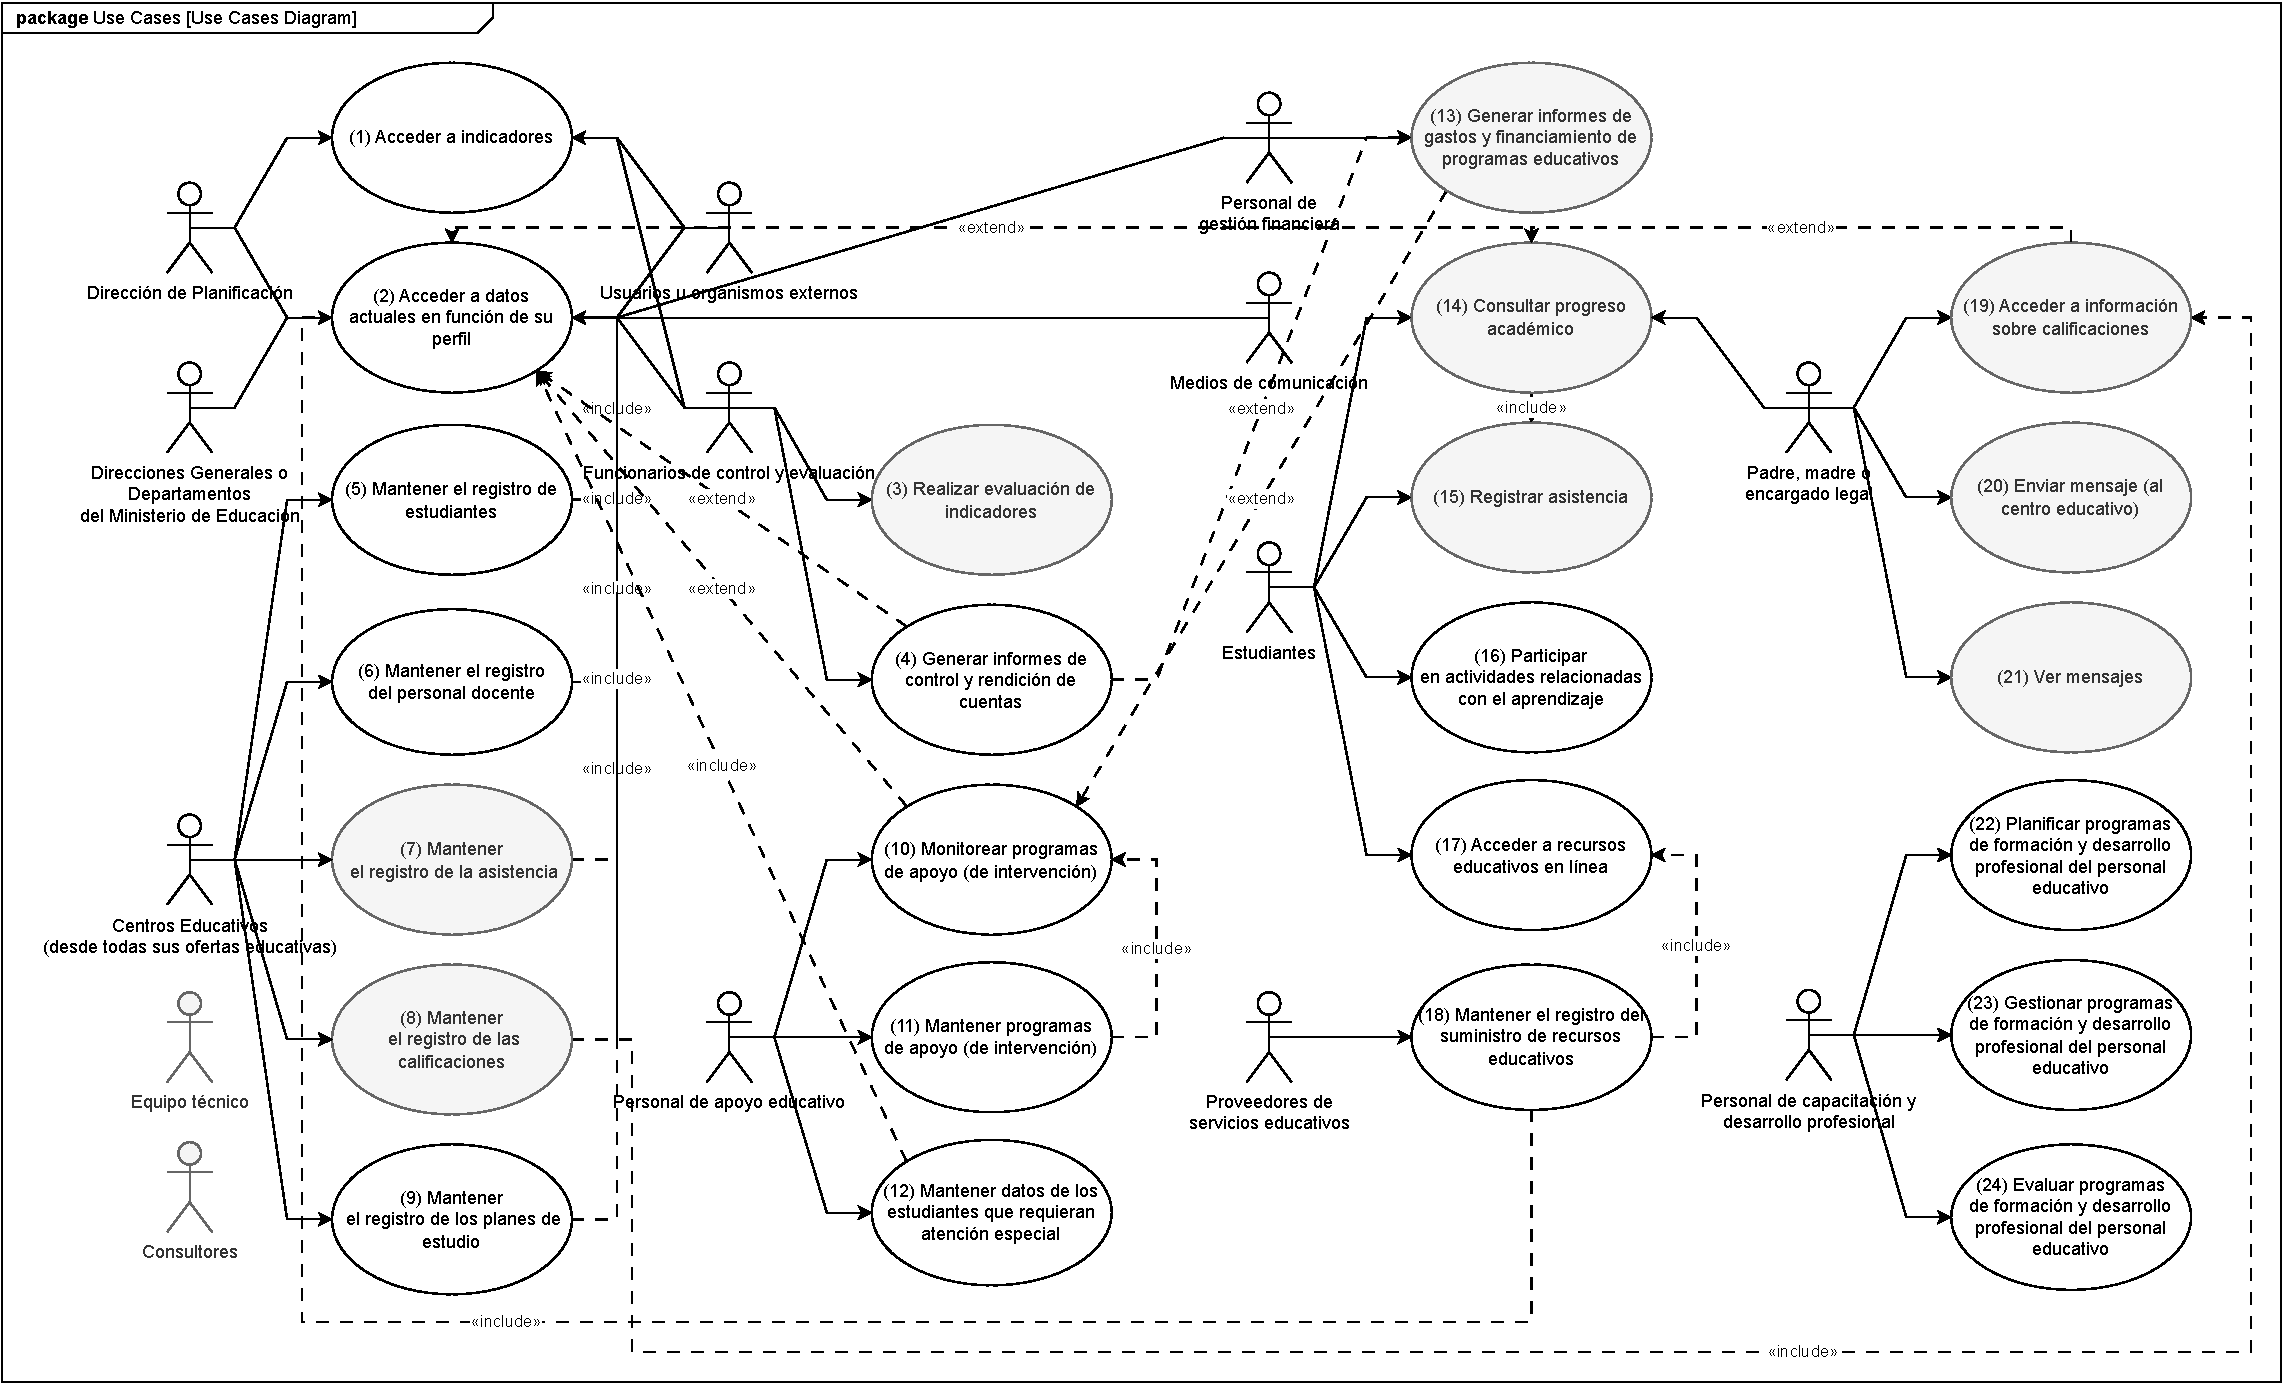
\includegraphics[width=\linewidth]{use} 
	\captionof{figure}{Diagrama de casos de uso. Cada monigote representa a un actor, y cada globo representa a un caso de uso. El conjunto de actores no se corresponde con el conjunto de entidades en el organigrama del ministerio. En el cuadro \ref{squ:workers}, a cada caso de uso se asigna un encargado que s\'i corresponde a una entidad en el organigrama del ministerio. Cada caso de uso de mantenimiento incluye las acciones ``cargar'', ``leer'', ``actualizar'' y ``eliminar''.}
	\label{fig:use}
 
 	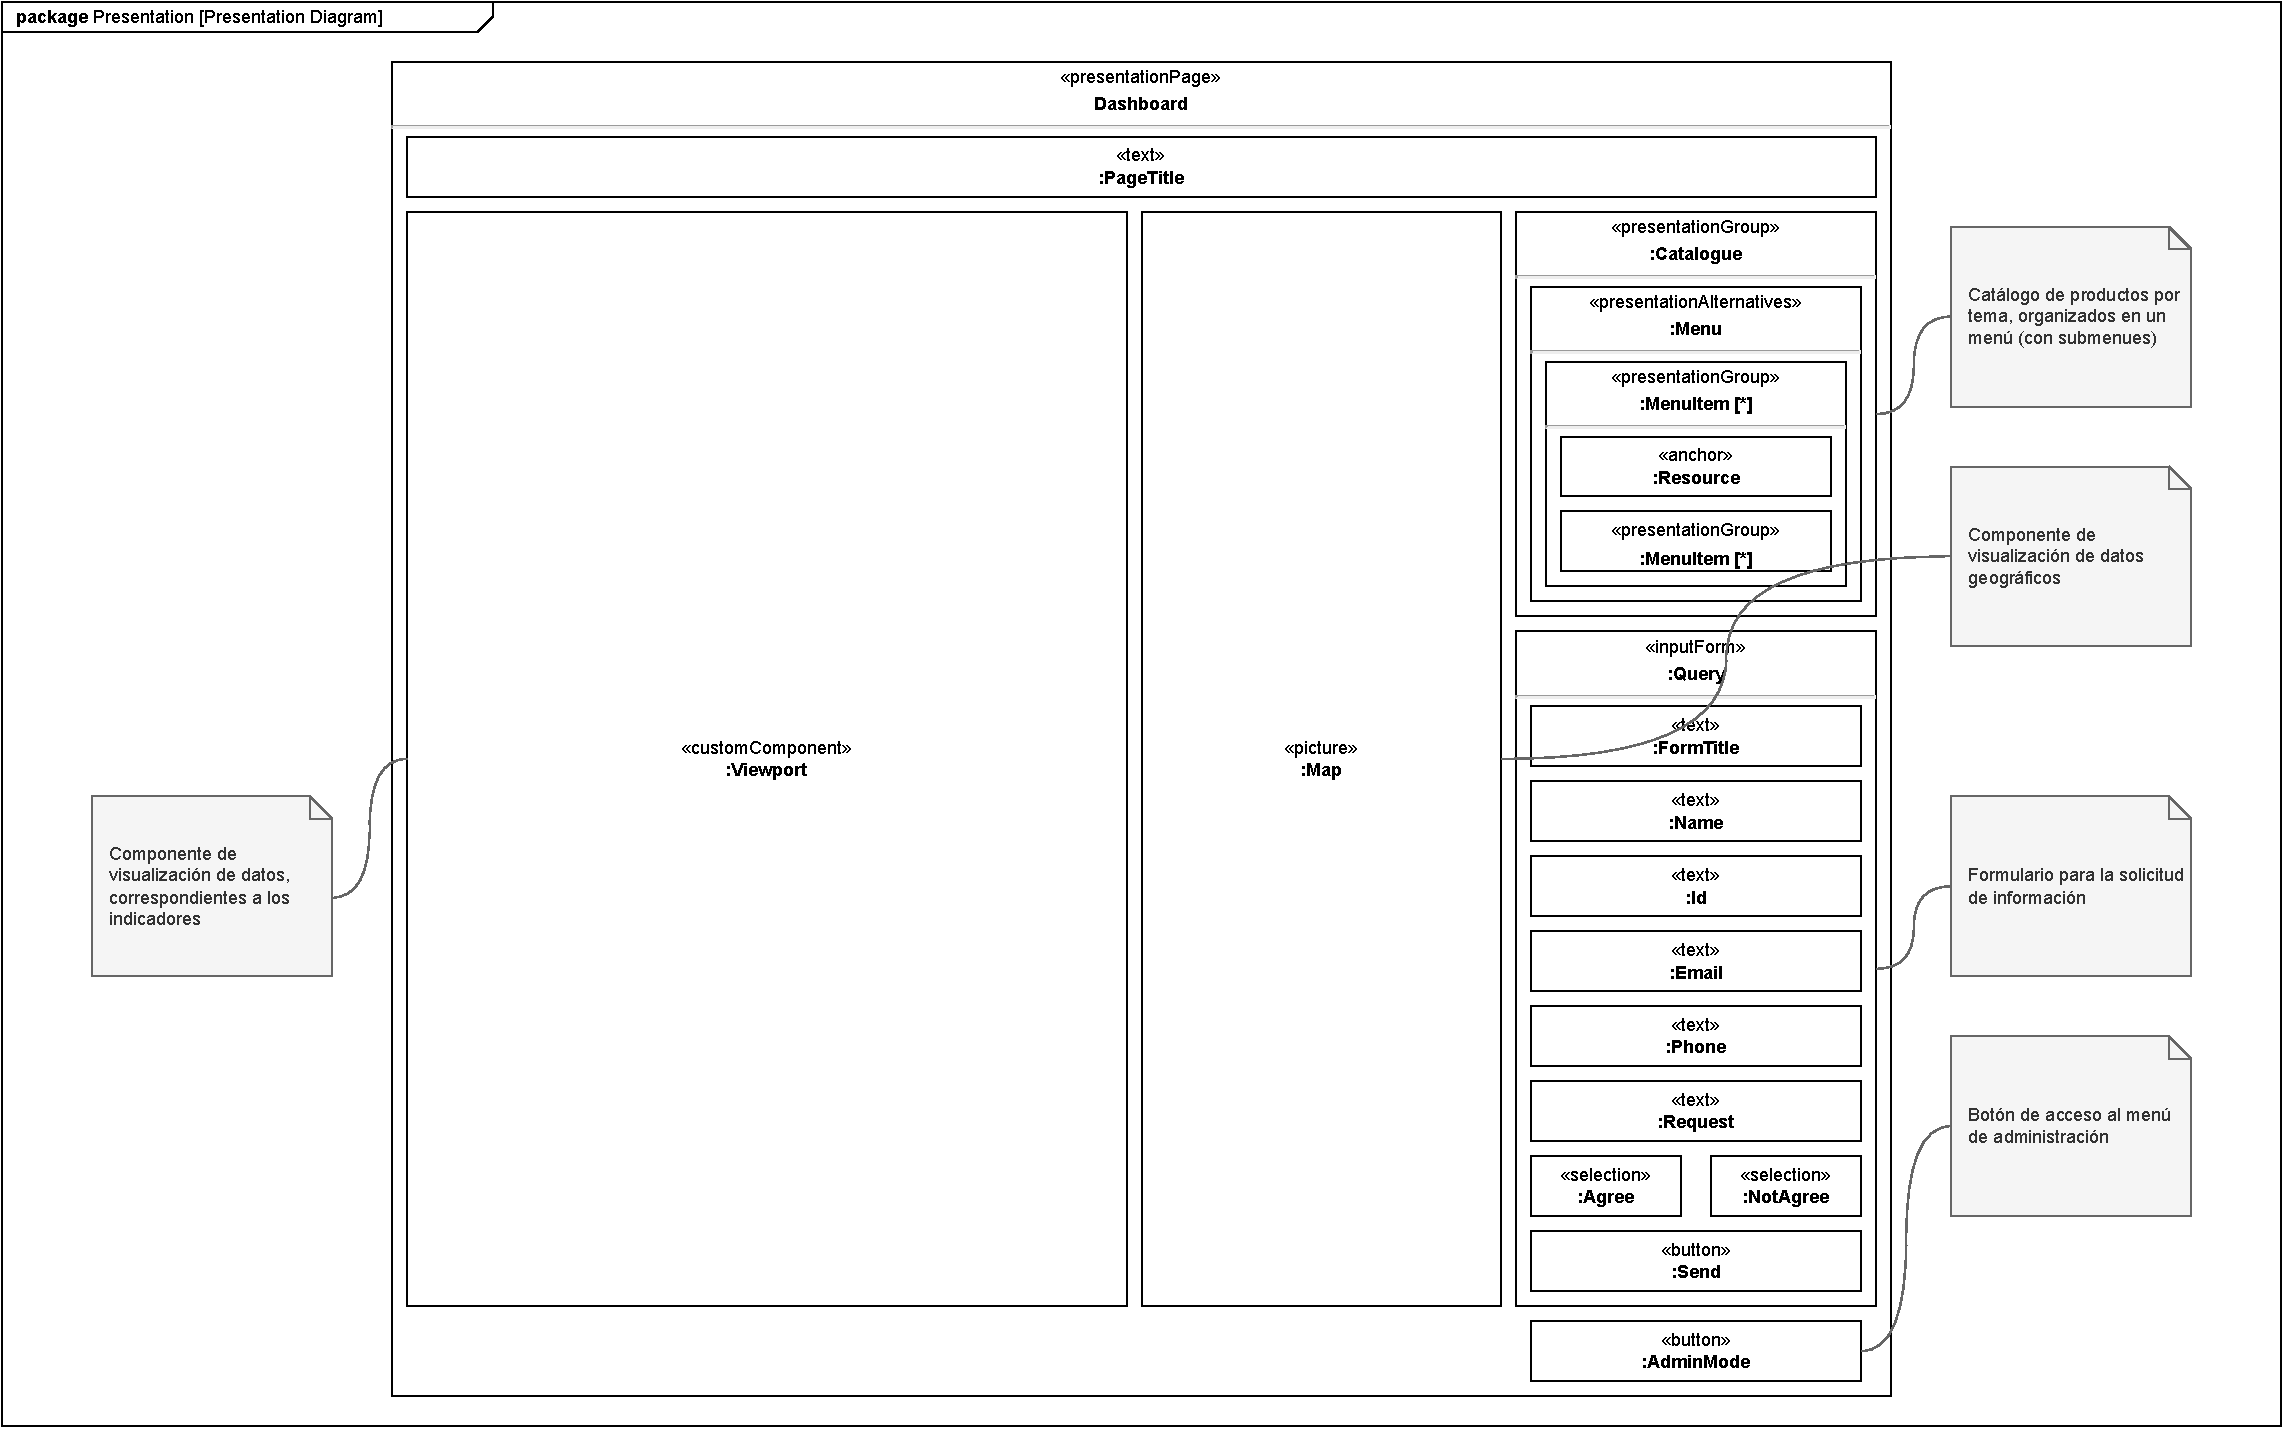
\includegraphics[width=\linewidth]{dashboard} 
 	\captionof{figure}{Diagrama presentaci\'on de la p\'agina de bienvenida.}
 	\label{fig:dash}
\end{minipage}%
\hspace{0.005\textwidth}
\begin{minipage}[b]{.685\textwidth}
 	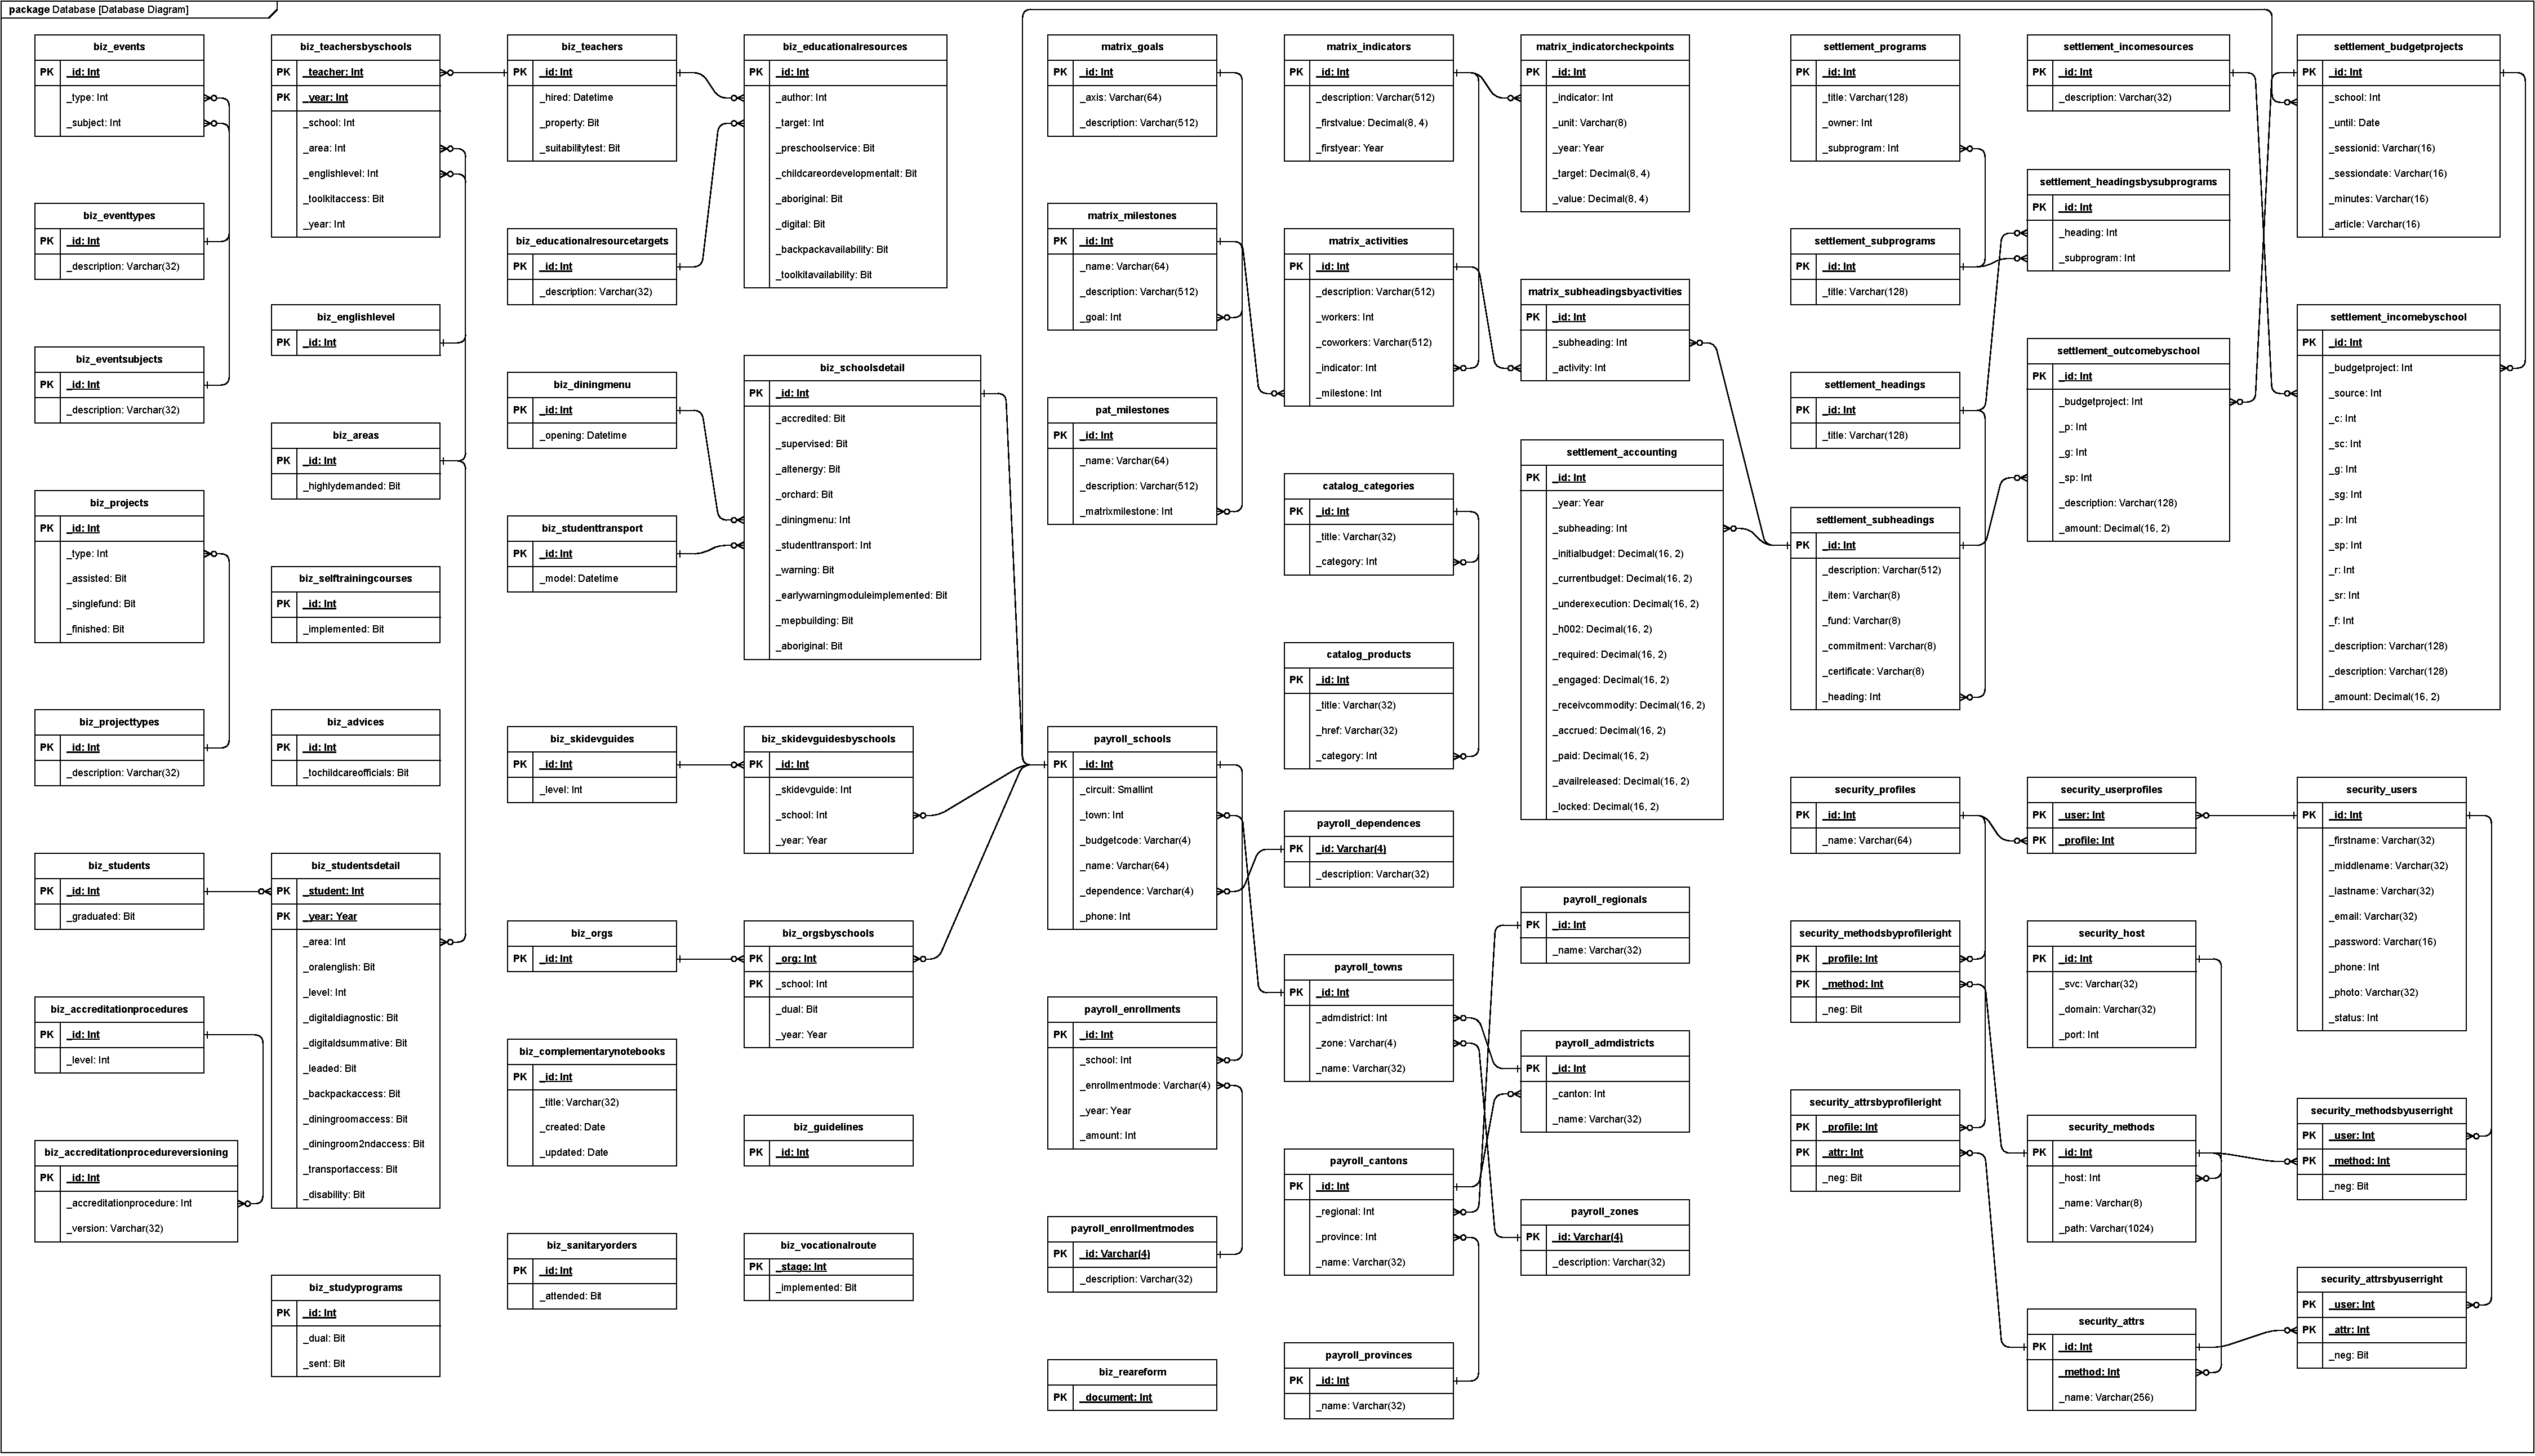
\includegraphics[width=\linewidth]{rem} 
 	\captionof{figure}{Diagrama de base de datos. Las tablas con prefijo ``payroll\_'', ``settlement\_'', ``matrix\_'', ``pat\_'', ``security\_'', ``biz\_'' y ``catalog\_'' corresponden a los m\'odulos de n\'omina de centros educativos, reporte de la liquidaci\'on general, indicadores, plan anual de trabajo (de centros educativos), seguridad, l\'ogica de negocio, y cat\'alogo de productos, respectivamente.}
 	\label{fig:rem}
\end{minipage}

% --------------------------------------------------------------------------------------------------------------------------------
%appendix
%section{Sem\'antica}



% --------------------------------------------------------------------------------------------------------------------------------
\end{document}
